% ABOUTME: Sequence models section of the IEEE report.
% ABOUTME: LSTM, temporal CNN and Transformer encoder: architectures, parameter counts, regularisation, CV results.
\section{Sequence Models}
\label{sec:dl-models}

Three networks read the sensor windows of Section~\ref{sec:dl-setup}
directly: an LSTM, a temporal convolutional network (TCN) and a Transformer
encoder. Each maps a window of 30 cycles of the 14 useful sensors to one
number, which the training loop multiplies by 125. None of them sees the
cycle number or the engineered features of Phase 1, so any skill they show
comes from the raw sensor history alone.

\subsection{Architectures}
\textbf{LSTM.} An LSTM~\cite{hochreiter1997lstm}, in the now standard form
with the forget gate of Gers et al.~\cite{gers2000forget}, reads the window
one cycle at a time. At cycle $t$ it combines the reading $x_t$ with the previous
hidden state $h_{t-1}$ through three gates and a candidate update,
\begin{align*}
f_t &= \sigma(W_f[h_{t-1}, x_t] + b_f), &
i_t &= \sigma(W_i[h_{t-1}, x_t] + b_i), \\
o_t &= \sigma(W_o[h_{t-1}, x_t] + b_o), &
g_t &= \tanh(W_g[h_{t-1}, x_t] + b_g), \\
c_t &= f_t \odot c_{t-1} + i_t \odot g_t, &
h_t &= o_t \odot \tanh(c_t).
\end{align*}
The cell state $c_t$ is updated by addition, so the gradient can flow back
across many cycles without vanishing. We stack one or two layers and pass
the hidden state after the last cycle through dropout to a linear output.

\textbf{Temporal CNN.} Following Bai et al.~\cite{bai2018tcn}, the TCN is a
stack of residual blocks. Each block applies two 1D convolutions with
kernel size $k = 3$, each followed by ReLU and dropout, and adds the block's
input back through a skip connection (a $1 \times 1$ convolution when the
channel count changes). The convolutions are causal: the input is padded on
the left only, so the output at cycle $t$ depends on cycles up to $t$ and
never on later ones. Block $j$ uses dilation $2^{j-1}$, so the gap between
the cycles one filter reads doubles from block to block. With $L$ blocks
the last output sees
\[
  R = 1 + 2(k-1)(2^{L}-1)
\]
cycles: 29 for three blocks and 61 for four. Three blocks therefore cover
29 of the 30 cycles in the window and four cover all of it. The output at
the last cycle feeds a linear layer.

\textbf{Transformer encoder.} Each cycle's 14 readings are projected to a
$d$-dimensional vector and a sinusoidal positional
encoding~\cite{vaswani2017attention} is added, followed by dropout. One or
two encoder layers follow, each with four attention heads, a feed-forward layer of width $4d$
and dropout. The 30 outputs are averaged and passed to a linear layer.
Self-attention and averaging both ignore the order of their inputs, so
without the positional encoding the model would give the same prediction for
a window and for the same window shuffled. It could not tell a rising
sensor from a falling one. The positional encoding gives each cycle a
distinct code, which the attention can use to recover order.

\subsection{Regularisation}
Every network is regularised in four ways. \emph{Dropout}~\cite{srivastava2014dropout}
sets a random fraction of activations to zero at each training step, so no
unit can rely on one particular partner, and turns off at prediction time.
\emph{Weight decay} adds $10^{-4}$ times the weights to every gradient
step, an L2 penalty that keeps the weights small. \emph{Gradient clipping}
rescales any gradient whose norm exceeds 1, so one batch with an unusually
large gradient, which recurrent networks occasionally produce, cannot swamp
the running averages that Adam uses to scale its steps. It does not limit
the capacity of the model.
\emph{Early stopping} ends training once the loss on the held-out
early-stopping engines has not improved for 10 epochs and restores the best
weights, so the number of epochs is chosen on engines the model was not
trained on.

\subsection{Tuning}
Each network is tuned with the five engine folds of Phase 1. For each one we
sample eight configurations, with seed 42, from a grid of 16 over width,
depth, dropout (0.1 or 0.3) and learning rate, and keep the configuration
with the lowest mean RMSE. Table~\ref{tab:dl-search} lists the grids and
the selected values. Adam, weight decay $10^{-4}$, batches of 256 and
patience 10 are fixed for every run.

\begin{table}[t]
\centering
\caption{Search spaces of the sequence models, eight of 16 configurations
sampled per network. Selected values are in parentheses.}
\label{tab:dl-search}
\footnotesize
\begin{tabular}{llp{3.2cm}}
\hline
Network & Hyperparameter & Values (selected) \\
\hline
LSTM & hidden size & 32, 64 (32) \\
 & layers & 1, 2 (1) \\
 & dropout & 0.1, 0.3 (0.3) \\
 & learning rate & 0.001, 0.003 (0.003) \\
\hline
TCN & channels & 32, 64 (64) \\
 & blocks & 3, 4 (4) \\
 & dropout & 0.1, 0.3 (0.1) \\
 & learning rate & 0.001, 0.003 (0.003) \\
\hline
Transformer & $d$ & 32, 64 (64) \\
 & layers & 1, 2 (1) \\
 & dropout & 0.1, 0.3 (0.1) \\
 & learning rate & 0.0003, 0.001 (0.001) \\
\hline
\end{tabular}
\end{table}

\subsection{Cross validation results}
Table~\ref{tab:dl-cv} puts the selected networks next to the Phase 1
models. Every row uses the same folds, the same scored cycles and RUL
capped at 125, but the training data differ: the networks train on 64 of
each fold's 80 training engines, because the other 16 are held out for
early stopping, while the Phase 1 models train on all 80. The networks
therefore learn from a fifth fewer engines but use those 16 to choose when
to stop, so the comparison is close but not exactly like for like. The
Transformer has the lowest error of any model in either
phase, 13.28 against 13.99 for XGBoost on engineered features. The LSTM
reaches 14.02 with 6{,}177 parameters, the fewest of the three networks.
The TCN is the weakest network at 15.91.

\begin{table}[t]
\centering
\caption{Five fold engine cross validation, RUL capped at 125. Late RMSE
covers cycles with true RUL $\le 50$. Phase 1 rows are from
Table~\ref{tab:cv-results}; those models train on 80 engines per fold,
the networks on 64.}
\label{tab:dl-cv}
\footnotesize
\setlength{\tabcolsep}{3pt}
\begin{tabular}{lrrrr}
\hline
Model (inputs) & Params & RMSE & MAE & Late RMSE \\
\hline
Transformer (windows) & 51{,}009 & 13.28 $\pm$ 0.34 & 9.54 & 7.98 \\
LSTM (windows) & 6{,}177 & 14.02 $\pm$ 0.43 & 10.00 & 8.84 \\
TCN (windows) & 90{,}241 & 15.91 $\pm$ 1.01 & 11.97 & 11.54 \\
\hline
XGBoost (engineered) & -- & 13.99 $\pm$ 0.46 & 9.81 & 9.88 \\
Random Forest (engineered) & -- & 14.42 $\pm$ 0.48 & 9.87 & 10.98 \\
XGBoost (raw) & -- & 16.42 $\pm$ 0.87 & 11.38 & 15.23 \\
\hline
\end{tabular}
\end{table}

The networks never see the cycle number or an engineered feature, so the
closest Phase 1 comparison is the raw feature set, where the best model
reaches 16.42 from the current cycle's readings and the cycle number. All
three networks do better, by 0.5 to 3.1 cycles, so the 30 cycle history
carries information that a single cycle does not. For the Transformer that
gain is larger than the 2.43 cycles the engineered features gave XGBoost.
Close to failure, only the Transformer and the LSTM beat XGBoost on
engineered features: on cycles with true RUL of at most 50 their RMSE is
7.98 and 8.84, against 9.88 for XGBoost and 11.54 for the TCN.

The search also shows three patterns, each from a few sampled
configurations. Every one layer LSTM beat both sampled two layer LSTMs, but
narrowly: 14.71 for the worst one layer configuration against 14.77 for the
better two layer one. Both sampled four block TCNs beat all six three block
TCNs by at least 1.4 cycles, but the fourth block adds depth and parameters
as well as the last cycle of the window, so the search cannot say which of
the two mattered. All three Transformers with dropout 0.3 were worse than
all five with dropout 0.1.

The Transformer's lead over XGBoost is 0.71 cycles, and the two models'
fold standard deviations are 0.34 and 0.46. Both models are the best of eight
configurations on these folds, so both scores are slightly optimistic, and
the test set gives the final ranking.

\subsection{Learning curves}
Fig.~\ref{fig:dl-curves} shows the training and early stopping losses of
each selected network on the first fold. For the LSTM and the Transformer
the early stopping loss stops improving at epochs 11 and 10 while the
training loss keeps falling slowly, but neither shows a sustained rise in
early stopping loss. The TCN does overfit: after epoch 7 its training loss
falls from 154 to 68 while its early stopping loss rises from 193 to between
210 and 355. Dropout of 0.1 does not prevent this. Early stopping limits
the damage by restoring the epoch 7 weights. Over all 24 configurations no
fold's best epoch is later than 35, so with a patience of 10 every run stops
by epoch 45 of the allowed 100.

\begin{figure*}[t]
\centering
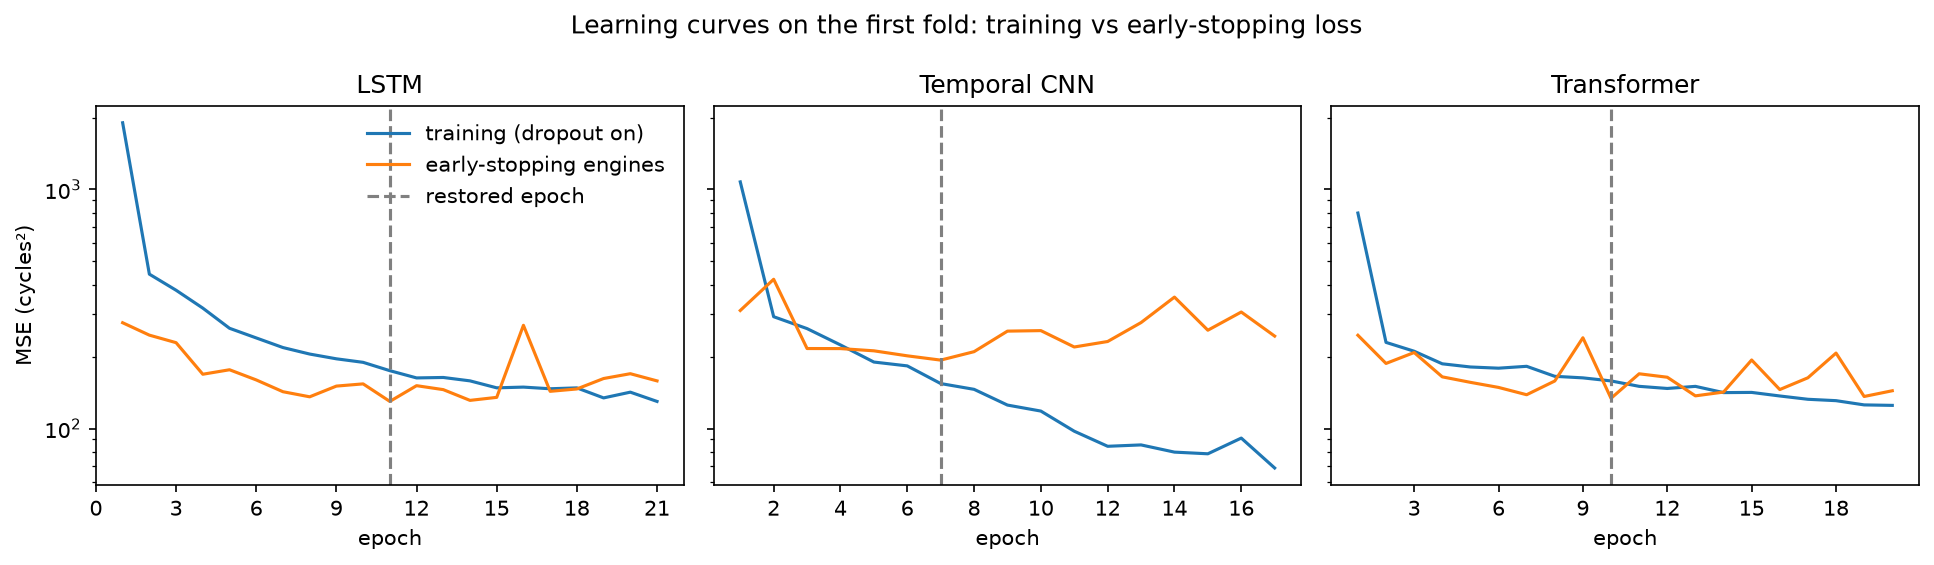
\includegraphics[width=\textwidth]{../figures/dl_learning_curves.png}
\caption{Training loss (dropout active) and early stopping loss of each
selected network on the first fold. The dashed line marks the epoch whose
weights are restored.}
\label{fig:dl-curves}
\end{figure*}
